\documentclass[a4paper,11pt]{article}
\usepackage[utf8]{inputenc}
\usepackage{textcomp}
\usepackage{lmodern}
\usepackage{listings}
\usepackage{graphicx}
\usepackage{listings}
\usepackage{color}
\definecolor{lightgray}{rgb}{0.9,0.9,0.9}
\definecolor{darkgray}{rgb}{0.4,0.4,0.4}
\definecolor{purple}{rgb}{0.65, 0.12, 0.82}
\usepackage{url}
\usepackage[top=3cm,bottom=3cm,left=3cm,right=3cm]{geometry}

\title{Royal Military Academy\\
	INFO-Y113 --- Management of Security: \\
	Concept Of Operations v2 \& Risk Analysis}

\author{DANHIER Pierre, LECOCQ Alexis, NYAKI Loïc}

\begin{document}
\maketitle
\newpage
\tableofcontents

\newpage

\section{Introduction}
In recent years, cyber-security has become a primary concern for companies all over the world. No matter the size of the company, data often represent the heart of their business and whether the concern is the secrecy of intellectual property, or users' privacy, the theft of private data bears a huge cost for companies. Be it a monetary cost (lawsuits, fines) or a reputation cost (loss of trust, public outrage). In the case of government agencies, states secrets and other classified information could be stolen by a foreign nation, possibly leading to the loss of lives in conflict zones, loss of political leverage on the international scene, domestic political turmoil and scandals or simply public embarrassment.\\

When trying to protect these sensitive data, a common measure is be to physically isolate the network from the internet, by creating an \textit{air gap}. Acting this way ensures that the data from the network is inaccessible from the outside world. The main issue with this method is that inevitably, some external data or files will at some point need to be imported into the secure network, be it for software update, or simply because some files from the outside are necessary for the people working in the secure network. In that case, a manual import (via USB drive, by connecting an external laptop into the secure network, or by using some other data transfer device) will be necessary.\\

The problem with that method is that it can compromise the security of the secure network. For instance, the data that is manually transferred into the network may have been infected by a malware, or the secure network might already be infected by a virus. In both cases, there is a possibility for some malicious code to exfiltrate data, or to spread a virus outside, by secretly writing on the device that was originally used to import the data into the network, such as USB drives or laptops.\\

As a consequence, we need to build a solution that prevents data leaks while allowing the transfer of files from the outside network into the secure network.

\section{Goals of the project}
\label{sec:goals}
Goals define the general direction of what the organization aims to accomplish, in the long term. Here, we wish to design a system that accomplishes three main goals :

\begin{enumerate}
\item{Create a device that completely prevents the exfiltration of data from a secure network, while allowing data to be transferred from the outside world into that secure network.}
\item{Ensure the availability of the system. The services should always be up, with no downtime}
\item{Allow specific users to manage and operate this system through an administration web page, accessible from within the secure network.}
\end{enumerate}

In this project, the general solution is imposed and should be a data diode, which will be described in section~\ref{sec:data-diode}.


\section{Objectives}
\label{sec:objectives}
Objectives can be considered as the building parts goals. They are concrete and can be achieved by following a certain number of steps. Achieving all the objectives should translate into achieving all the goals.\\


We identify the following general objectives:
\begin{itemize}
\item{Build a web interface for administrating the data diode}
\item{Use the File Transfer Protocol to implement a file transfer functionality between the outside network and the secure network.}
\end{itemize}

The next sections identify more specific objectives.

\subsection{Data Confidentiality}
There should be no way for data to leak outside of the secure network. Preventing physical access to a computer in the secure network is out of the scope of this project (see section \ref{sec:outscope}).\\

The objectives for ensuring data confidentiality are as follows:

\begin{itemize}
\item{Physically prevent data from exiting the secure network}
\item{When establishing communication with the system, user credentials and information shouldn't be exposed to other users.}
\end{itemize}

\subsection{Data Integrity}
The data retrieved from the outside of the network should be the same as the data that was initially sent. No data corruption or modification should take place.

\subsection{System Availability}
The system should always be up, unless it is turned off on purpose by a legitimate user or administrator.

The objectives for ensuring system availability are as follows:

\begin{itemize}
\item{The system must keep working no matter how many files are pushed onto the system}
\item{An authorized user should always be able to transfer a file into the secure network}
\item{An authorized user should always be able to access and operate the administration page}
\item{In case of system crash, the system must restarted immediately}
\item{The web interface should always be accessible and working as intended. Therefore, measures should be taken against Cross site scripting (XSS) and Cross Site Request Forgery attacks (CSRF).}

\end{itemize}


\section{Scope}
It is important to precisely identify the scope of this project, in relation to our goals and objectives.\\

Our solution is destined to be integrated in an existing system. As such, when considering the security of the system as a whole, we must identify which security aspects fall under our responsibility and which don't. 

\subsection{In scope}
The following elements are in scope, which means that it is our responsibility to make sure that the security of these elements is ensured.

\begin{itemize}
\item{The availability of the file transfer service}
\item{The confidentiality of user data and credentials when interacting with the data diode (see section \ref{sec:data-diode})}
\item{The confidentiality of the data within the secure network. There should be no data leak.}
\item{The integrity of the data pushed through the data diode}
\end{itemize}

\subsection{Out of scope}
\label{sec:outscope}
The following elements are out of scope. This means that the security of these elements does not fall under our responsibility, but rather under the responsibility of the client, or another third party.

\begin{itemize}
\item{The physical access to the hardware, such as the power button or Ethernet cables}
\item{The physical integrity of the hardware}
\item{The electrical power source}
\item{The security within the secure network, such as the presence of malwares or other viruses}
\end{itemize}


\section{Data Diode}
\label{sec:data-diode}
Based on the goals and objectives specified respectively in section \ref{sec:goals} and section \ref{sec:objectives} and on the project requirements, we are going to implement a \textit{data diode}.\\

Just like a diode only conduct current in one direction, a data diode is a networking device that only allows data to flow in one direction. It is composed of two physical servers: one server communicates with the outside network and the other one communicate with the secure network. The two servers are connected together by a single unidirectional fiber optics cable.\\

A fiber optic connection normally uses two cables: one for each direction. In the case of 	 data diode, only one cable is used, allowing the data to flow in one direction. The cable going in the other direction is physically cut. As a consequence, data going through a data diode can only flow in one direction, which is required by the goals defined in section \ref{sec:goals}.\\

The one-way communication channel between the two sides of the data-diode forbids the use of usual TCP based protocols (such as HTTP or FTP), as TCP requires bi-directional communication between two parties. As data between the two sides of the data-diode can only flow in one direction, we need data to be send over a protocol that doesn't require bi-directional communication. This can be done by using UDP for the communication between our two servers.\\

However UDP comes with its own limitations, as it doesn't ensure the order at which the paquets arrive, nor does it manage packets loss. These issues will therefore need to be taken into account at the software level.


\begin{figure}
	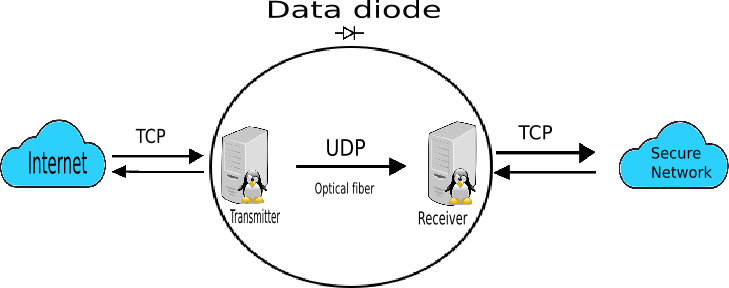
\includegraphics[scale=0.7]{img/network.png}
	\caption{High level architecture of a data diode.}
\end{figure}


\subsection{Applications}
With this data diode, we decided to keep things simple and to focus on proposing the two following services: a File Transfer service, as well as a data-diode administration service, as specified in our goals and objectives (section \ref{sec:goals} and section \ref{sec:objectives}).\\

Other applications such as email management and web browsing will be considered for future versions of the data-diode.

\subsubsection{File Transfer (FTP)}
The main application of this project is a file transfer service that will enable files to be pushed from the outside network into a directory situated in the inner part of the data diode, through the use of the File Transfer Protocol (FTP). That directory will be referred as the \textit{download directory}\\

The management of the FTP accounts is handled by administrators through the data diode administration page, as described in section \ref{sec:administration}.

\subsubsection{Administration and User Management}
\label{sec:administration}
One of the goals of this project is the creation of a web interface for managing the data diode. We will implement an HTTP server, on the internal side of the data diode. This administration interface will allow administrators:

\begin{itemize}
\item{Monitor file transfers: the administrator should be able to see what files have been transferred, or see if there has been issues regarding the transfer of a file}
\item{Create or delete FTP accounts}
\item{Start, stop or restart the data-diode}
\item{Purge \textit{download directory}}
\item{Set or modify the maximum size of the \textit{download directory}}
\end{itemize} 


\subsection{Physical Architecture}
The data diode is composed of two separate servers connected to each other through a unidirectional fiber optics cable. The server facing the outside network is called \textit{the sender}, the server facing the secure network is called \textit{the receiver}.\\

Each server contains the following components :
\begin{itemize}
\item{Two network interfaces: one for connecting to a network, and one for connecting to the other server}
\item{A fiber optic adapter, to translate the signal coming from the fiber optic cable from light into a signal that can be transmitted through an Ethernet port.}
\end{itemize}

\subsection{Software architecture}
The data diode is composed of two servers, \textit{the sender} and \textit{the receiver}, which have different roles. 

\subsubsection{The Sender}
The \textit{sender} must be able to receive FTP PUT requests from the outside network and to transmit data to the \textit{receiver} via UDP.\\

The sender must therefore be comprised of :
\begin{itemize}
\item{A FTP server}
\item{A UDP client}
\end{itemize} 

\subsubsection{The Receiver}
The \textit{receiver} must be able to receive UDP paquets and reconstruct them as a file that will be placed in a specific directory. Moreover, a web server must be running on the machine in order to enable the administration page.\\

In summary, the receiver will contain :
\begin{itemize}
\item{A UDP server}
\item{A web server}
\end{itemize}

\subsection{Simulating a data diode}
At first, instead of using a real data diode, we are going to build the prototype of a data diode by simulating the actual system through software. The unidirectional nature of the data transfer will be simulated by modifying the IP table in a way that will allow traffic in one direction, and drop all traffic going in the other direction.


\section{Users}
We identify three types of users : the administrators, the simple users and the FTP users.

\subsection{Simple Users}
Simple users are users from inside the secure network. Their main interaction with the system is that they will need to retrieve the files from the \textit{download directory}, by accessing the web interface. They do no possess other privileges than that.

\subsection{Administrators}
The role of the administrators is to manage the system so that it runs smoothly. They have access to all the functionalities of the administration interface as described in section \ref{sec:administration}.

\subsection{FTP Users}
FTP users operate from outside the secure network and are allowed to push files into the secure network. Each FTP user will have an account on the data diode, created by an administrator. This account allows him to push data through the data diode, via an FTP connection.

\section{Administration and Management}
\subsection{Users Administration}
The administration interface allows administrators to manage the user that can access the data diode. The users from outside of the data diode are responsible for pushing files into the \textit{download directory}. The user from the inside of the secure network will then access the web interface to retrieve the files they want on their computer.

\subsubsection{Administration of Simple Users}
We decide that every user inside the secure network should be able to access the files that have been imported into the \textit{download directory}. Therefore, there will be no specific management of these users.

\subsubsection{Administrators of other Administrators}
Administrators are able to create an administrator account, or to suspend the account of another administrator.

\subsection{Data Diode Installation, Configuration and Administration}

\subsubsection{Installation}
The data diode is provided to the client with the programs already installed, and a default administrator account. At first use, the password should be modified.

\subsubsection{Configuration}
The data diode settings will be specified in a configuration file that can be modified manually. The settings include the HTTP port that must be used, and the maximum size of the \textit{download directory}.

\subsubsection{Administration}
\section{Risk analysis}
\subsection{Hardware}
\subsubsection{Source}
Someone malicious manage to get physical access to the data-diode. The hacker can then branch a device to the data diode to read or send packets to the data diode.
\subsubsection{Threats}
The hacker can
\begin{itemize}
\item shut down the system or make a direct DDOS attack causing the loss of availability of the system.
\item read or modify the files send to the data diode. The integrity and confidentiality are then corrupted
\item block files before reaching the data diode.
\end{itemize}
\subsubsection{Countermeasures}
The physical access to the system is out of our scope. The risk is then tranfered to the client. However, the risk for the integrity and confidentiality of the system is mitigated by the use of cryptography.
\subsection{Secure network}
\subsubsection{Source}
An unauthorized person connects into the secure network.
\subsubsection{Threats}
This person can then use packet sniffing techniques to read credentials and then try to connect to the data diode with a user or administrator account.
\subsubsection{Countermeasures}
As well as the physical access to the data diode, the integrity of the secure network is out of our scope but the use of cryptography mitigate the risk.
\subsection{External network}
\subsubsection{Source}
An opponent take knowledge of the IP adress of the data diode.
\subsubsection{Threats}
He can then launch a DDOS attack against the system by floating the identification process with fake connection demands. The availability of the system can then be endangered.
\subsubsection{Countermeasures}
When the system detects that a certain IP adress unsuccessfully tries to connect itself to the data diode a certain amount of times, we can temporarily ban this IP adress from the access to our system.  The risk is then mitigated.
\subsubsection{Residual risk}
If the opponent has access to a botnet with enough different IP adresses, he still can DDOS attack our sytem with success. The availability of our sytem could then be suspended.
\subsection{Administration webpage}
\subsubsection{Source}
Someone inside the secure network who has not the administrator status wants to obtain this right.
\subsubsection{Threats}
This person can use SQL injections or try to brute force an administrator account through the login webpage. The brute force attack can endanger the availability of the system. If the opponent manage to get an administrator account he can turn off the data diode or modify users privileges and accounts.
\subsubsection{Countermeasures}
We can avoid these risks by preventing SQL injections in the source code of the login webpage and by detecting unsuccessful connection attempts. After a certain amount of failed connections by the IP adress, the system bans this adress.
\subsection{Users}
\subsubsection{Source}
A system halt during the creation or modification of a user profile gives rights to this user that he should not have.
\subsubsection{Threats}
This user can obtain the administrator status if the systems creates a user with full rights and then reduces the rights. If the system halts before or during the restrictions, the user can remain with certain rights he should not have.
\subsubsection{Countermeasures}
We avoid this risk by creating users with no rights and then allow him some of them. If the system halts before the end of the creation or modification, the user has no rights he should no have.  
\subsection{FTP servers}
\subsubsection{Source}
A provider push so many files that the data diode cannot store them all.
\subsubsection{Threat}
A provider can lauch a "DDOS attack" by sending a lot of small files or some really big files.
\subsubsection{Countermeasure}
When a user send a certain amount of data, he needs to wait before sending again some new data. That prevents the "DDOS attack" risk and mitigate the starving risk for other users.



\end{document}
